\chapter{Resultados}
\label{chap:resultados}

Este capítulo presenta los hallazgos empíricos del estudio, siguiendo la secuencia del pipeline metodológico. Se inicia con la caracterización de la cohorte y el análisis de la variabilidad de los datos, lo cual fundamenta las decisiones de preprocesamiento. A continuación, se detalla el proceso de establecimiento de la ``verdad operativa'' mediante el análisis de conglomerados. Posteriormente, se presenta el rendimiento del sistema de inferencia difusa en su validación contra esta referencia. Finalmente, se expone un análisis de robustez que revela la contribución sinérgica de las variables al modelo.

% ============================================================================
\section{Caracterización de la Cohorte y Análisis de Variabilidad de Datos}
\label{sec:caracterizacion_cohorte}
% ============================================================================

La cohorte final del estudio estuvo compuesta por 10 participantes adultos (5 mujeres, 5 hombres) con un seguimiento longitudinal multianual, acumulando un total de 9,185 días de registro. Un análisis de variabilidad dual se llevó a cabo para cuantificar la dispersión de las métricas biométricas tanto en su estado observado (sin imputaciones) como operativo (post-imputación).

Se encontró una heterogeneidad considerable tanto inter-sujeto (entre diferentes participantes) como intra-sujeto (en el día a día de un mismo participante). El coeficiente de variación (CV) para métricas clave como los minutos de ejercicio diario superó el 100\%, indicando una alta irregularidad en los patrones de actividad.

\begin{figure}[htbp]
    \centering
    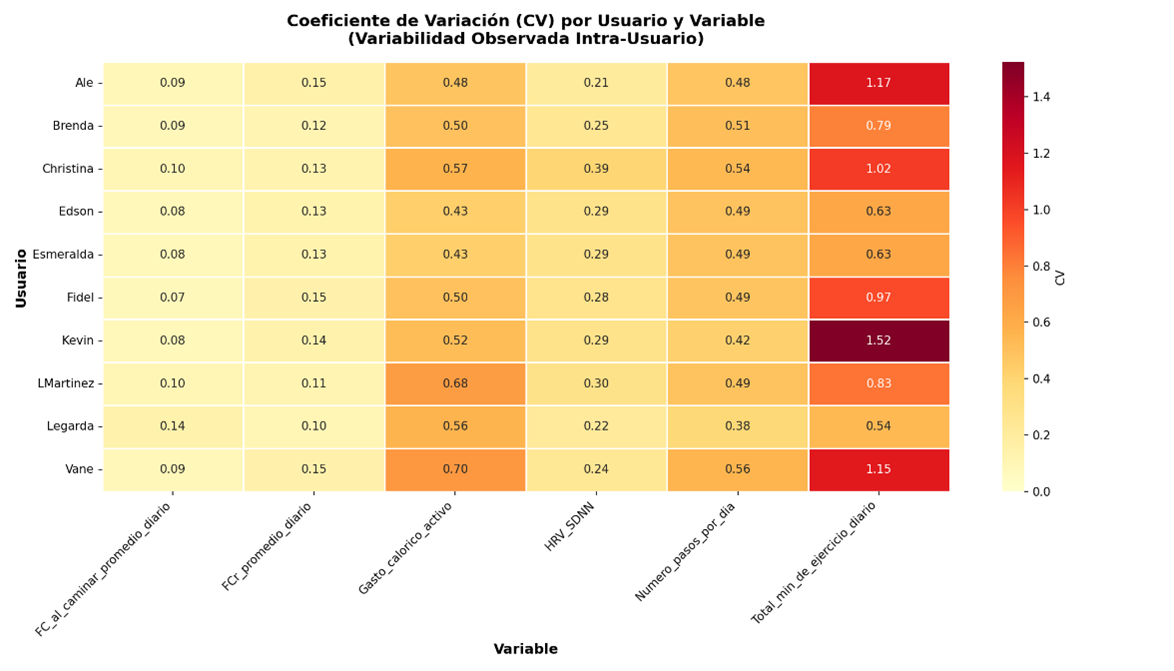
\includegraphics[width=0.95\textwidth]{figuras/coeficiente_de_variacion.png}
    \caption{Mapa de calor de variabilidad (Coeficiente de Variación) por usuario y variable}
    \label{fig:mapa_calor_variabilidad}
\end{figure}

Como se observa en el mapa de calor de variabilidad, algunos usuarios exhiben patrones más consistentes (CV más bajos) que otros. De igual manera, la comparación entre la variabilidad de los datos puramente observados y la de los datos operativos post-imputación mostró que el proceso de imputación, si bien necesario, tiende a reducir la dispersión de algunas variables como la HRV\_SDNN y la FCr\_promedio\_diario, mientras que la incrementa ligeramente en otras.

\begin{figure}[htbp]
    \centering
    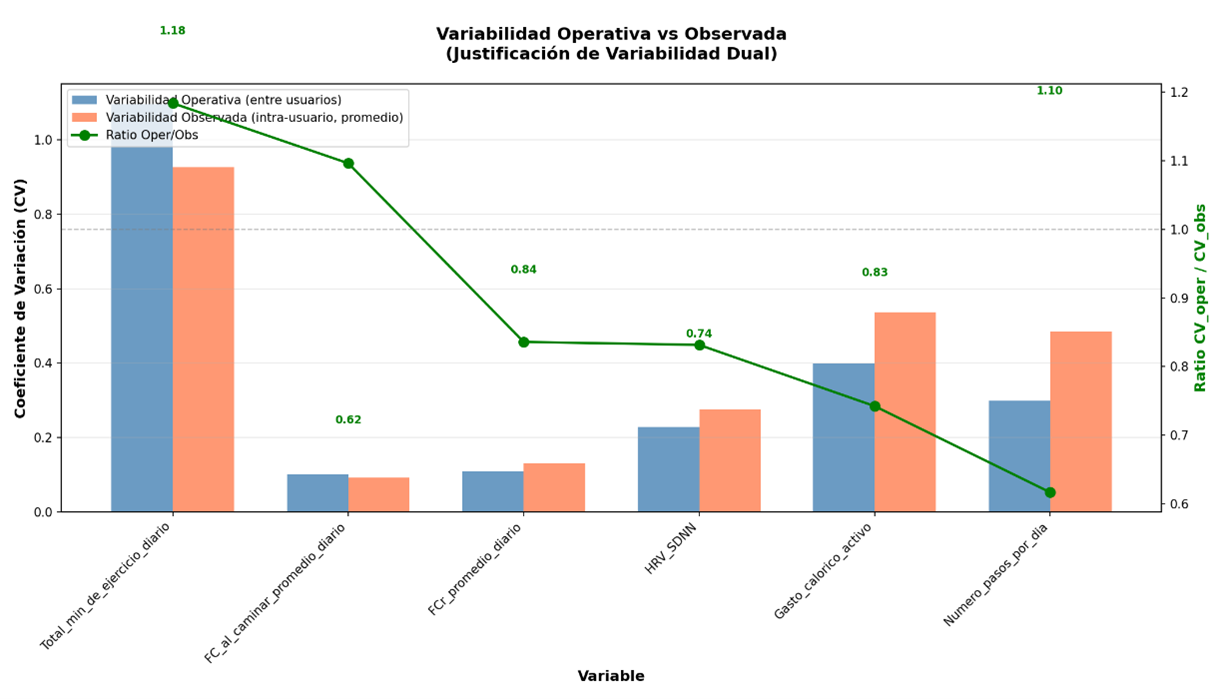
\includegraphics[width=0.95\textwidth]{figuras/variabilidadoperativa_vs_observada.png}
    \caption{Comparación de variabilidad entre datos observados y operativos (post-imputación)}
    \label{fig:variabilidad_comparativa}
\end{figure}

Esta alta variabilidad natural de los datos recopilados en condiciones de vida libre justificó la decisión metodológica de agregar los datos a nivel semanal utilizando estadísticos robustos (mediana e IQR), con el fin de amortiguar el ruido diario y analizar patrones de comportamiento más estables y sostenidos.

% ============================================================================
\section{Establecimiento de la Verdad Operativa: Análisis de Conglomerados}
\label{sec:verdad_operativa_clustering}
% ============================================================================

Previo al análisis de conglomerados, se verificó la ausencia de multicolinealidad severa entre las ocho características semanales seleccionadas. Todas las variables presentaron un Factor de Inflación de la Varianza (VIF) inferior a 2.0, lo que confirma su idoneidad para el modelado.

\begin{figure}[htbp]
    \centering
    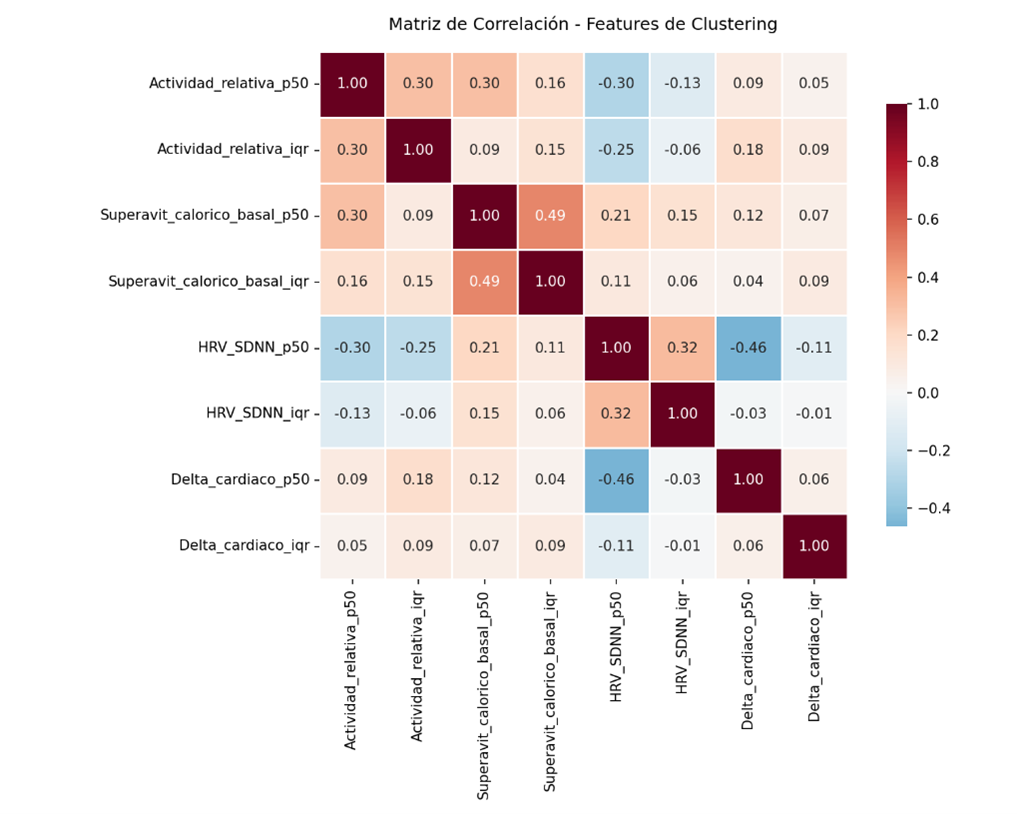
\includegraphics[width=0.85\textwidth]{figuras/matriz_correlacion_features_clustering.png}
    \caption{Matriz de correlación de características para clustering (verificación de multicolinealidad)}
    \label{fig:matriz_correlacion}
\end{figure}

Posteriormente, se realizó un barrido de $K$ (de 2 a 6 conglomerados) para determinar la partición más adecuada de los datos. El coeficiente de Silhouette alcanzó su máximo en $K=2$, indicando que la estructura más clara y estable en los datos correspondía a dos perfiles de comportamiento distintos.

\begin{figure}[htbp]
    \centering
    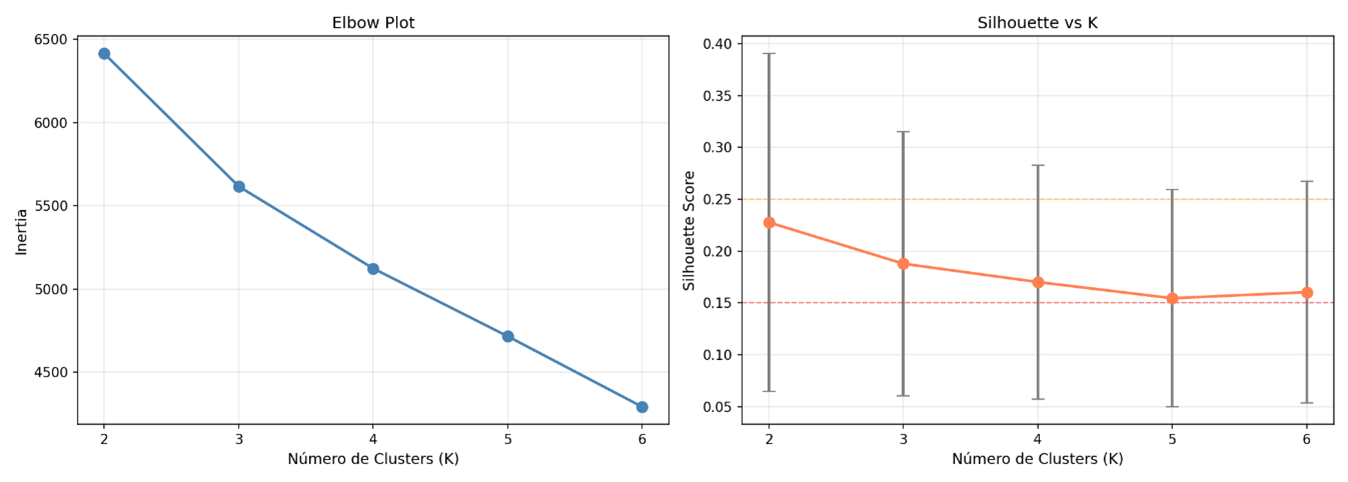
\includegraphics[width=0.9\textwidth]{figuras/PCA_elbow_vs_shilloete.png}
    \caption{Análisis de determinación de K óptimo: Método del codo (Elbow) y Coeficiente de Silhouette}
    \label{fig:silhouette_elbow}
\end{figure}

El análisis de componentes principales (PCA) confirmó visualmente la tendencia de los datos a separarse en dos grupos a lo largo del primer componente principal, el cual estaba fuertemente influenciado por las variables de actividad y gasto calórico.

\begin{figure}[htbp]
    \centering
    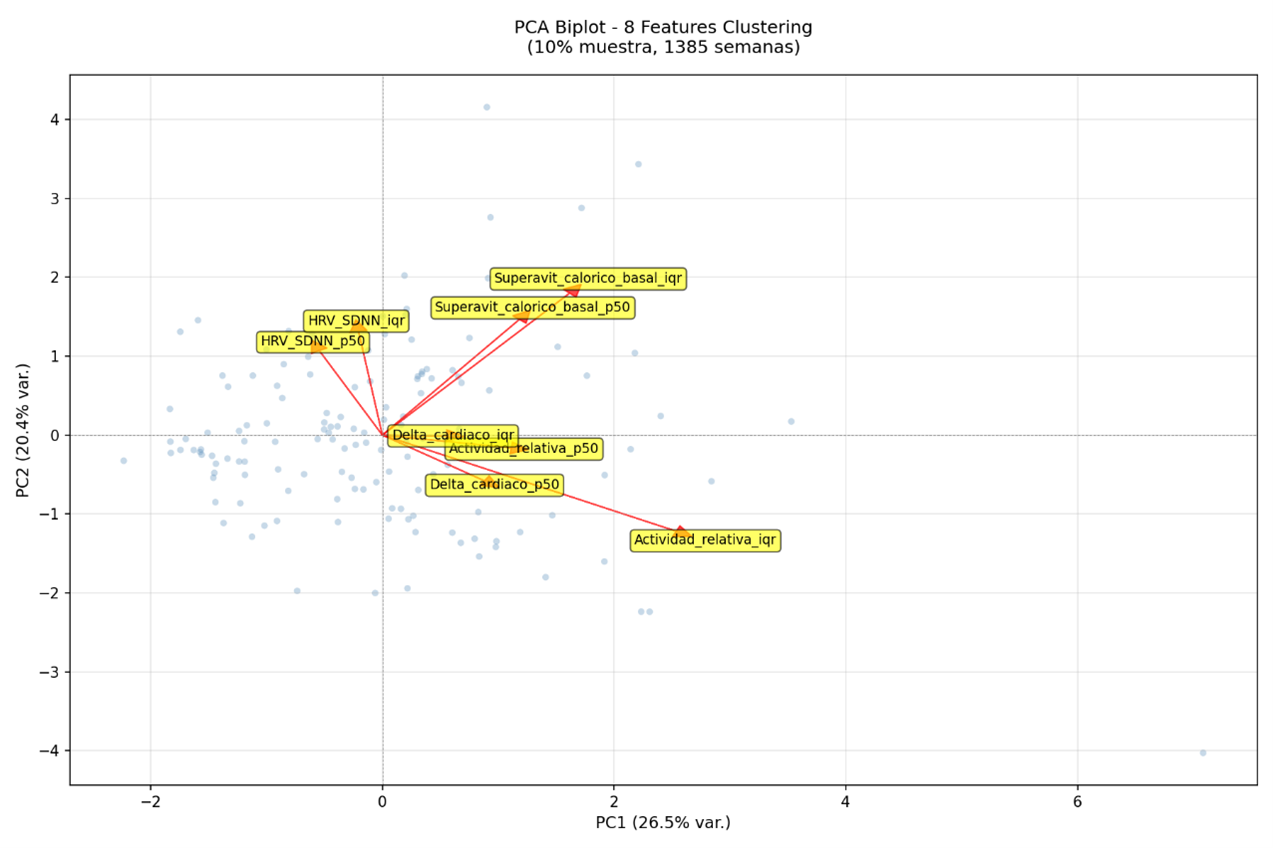
\includegraphics[width=0.95\textwidth]{figuras/PCA_biplot.png}
    \caption{Análisis de Componentes Principales (PCA) mostrando la separación en dos conglomerados}
    \label{fig:pca_biplot}
\end{figure}

Los perfiles de estos dos conglomerados se analizaron estadísticamente para su caracterización clínica. El Conglomerado 0 (``Bajo Sedentarismo'') presentó valores de mediana significativamente más altos en Actividad\_relativa\_p50 y Superavit\_calorico\_basal\_p50 en comparación con el Conglomerado 1 (``Alto Sedentarismo''). Las diferencias fueron estadísticamente irrefutables ($p < .001$) y con un tamaño del efecto grande (Cohen's $d > 0.9$). Curiosamente, la HRV\_SDNN no mostró una diferencia significativa entre ambos grupos.

\begin{figure}[htbp]
    \centering
    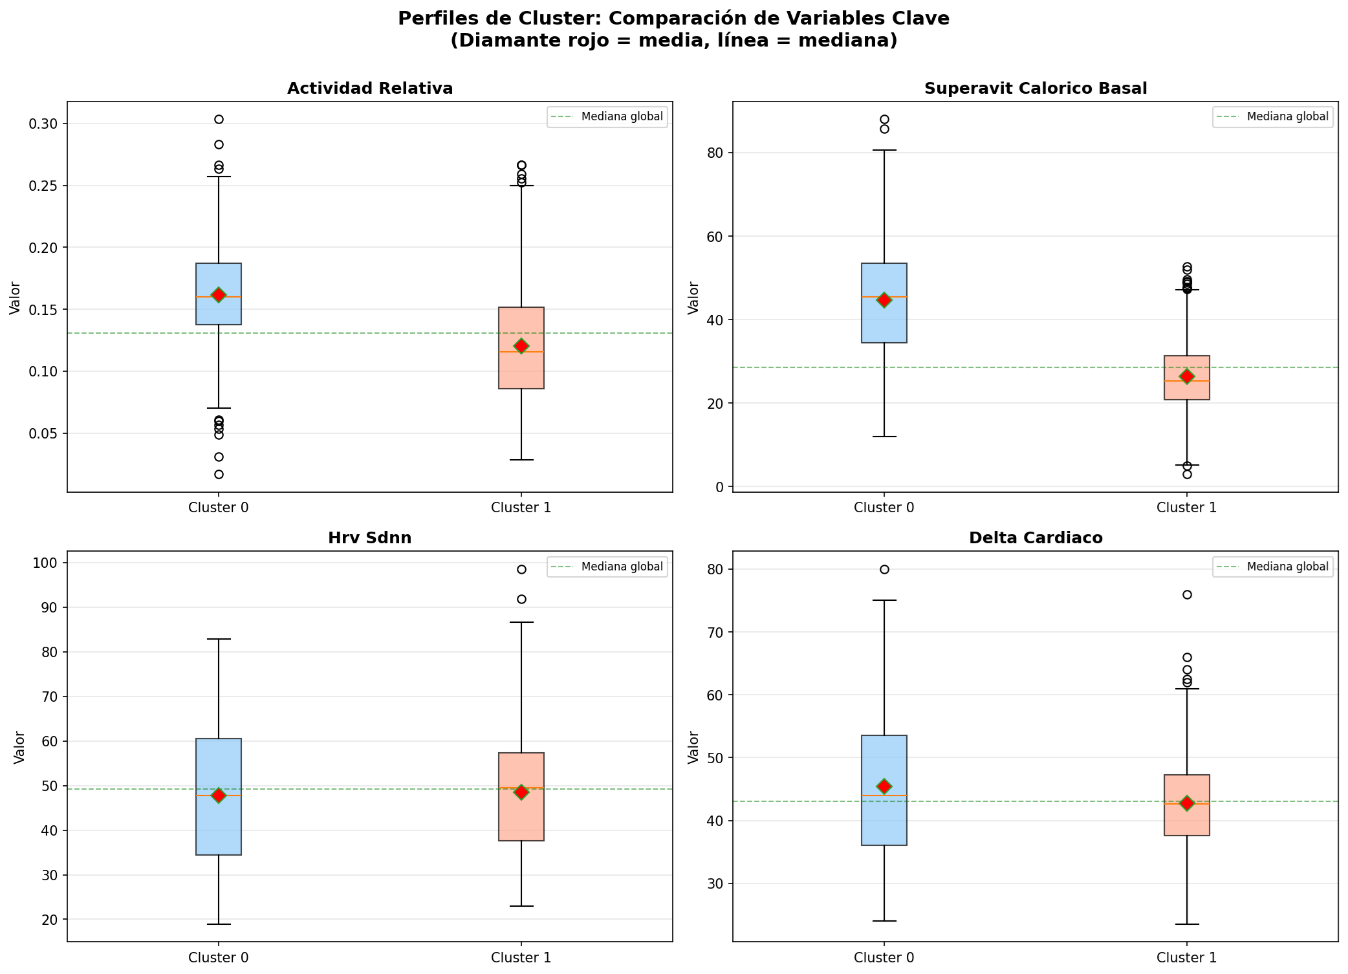
\includegraphics[width=0.95\textwidth]{figuras/perfiles_de_clusters.png}
    \caption{Perfiles de los dos conglomerados según las 4 variables principales (Actividad relativa, Superávit calórico, HRV-SDNN, Delta cardíaco)}
    \label{fig:perfiles_clusters}
\end{figure}

La \Cref{tab:distribucion_clusters_usuario} muestra la distribución de semanas asignadas a cada conglomerado por usuario.

\begin{table}[htbp]
\centering
\caption{Distribución de Semanas por Conglomerado y Usuario}
\label{tab:distribucion_clusters_usuario}
\small
\begin{tabular}{@{}lcccr@{}}
\toprule
\textbf{Usuario} & \textbf{Cluster Alto Sed (\%)} & \textbf{Cluster Bajo Sed (\%)} & \textbf{Diferencia absoluta (\%)} \\
\midrule
u1  & 99.3 & 0.7  & 98.7 \\
u2  & 85.7 & 14.3 & 71.4 \\
u3  & 11.3 & 88.7 & 77.3 \\
u4  & 71.4 & 28.6 & 42.9 \\
u5  & 64.3 & 35.7 & 28.6 \\
u6  & 82.0 & 18.0 & 64.0 \\
u7  & 94.7 & 5.3  & 89.5 \\
u8  & 27.7 & 72.3 & 44.5 \\
u9  & 84.2 & 15.8 & 68.5 \\
u10 & 80.9 & 19.1 & 61.8 \\
\bottomrule
\end{tabular}
\end{table}

La asignación de cada una de las 1,337 semanas válidas a uno de estos dos conglomerados se constituyó como la ``verdad operativa'': una clasificación objetiva y empírica utilizada como referencia para la validación del sistema de inferencia difusa.

% ============================================================================
\section{Rendimiento del Sistema de Inferencia Difusa}
\label{sec:rendimiento_sistema_difuso}
% ============================================================================

El rendimiento del modelo difuso se evaluó mediante su concordancia con la clasificación de la verdad operativa. Tras una búsqueda del umbral de decisión ($\tau$) que maximizara el F1-Score, se estableció un valor óptimo de $\tau = 0.30$. Con este umbral, el sistema difuso alcanzó un rendimiento global robusto, con un F1-Score de 0.840, una Exactitud de 0.740 y una alta Sensibilidad (Recall) de 0.976.

El análisis por participante reveló una heterogeneidad en el rendimiento, con un F1-Score que osciló entre 0.215 y 0.997. Usuarios con patrones de comportamiento más estables mostraron una concordancia muy alta (ej. u1, u7), mientras que aquellos con mayor variabilidad intra-semanal presentaron mayores discrepancias, evidenciando áreas de oportunidad para la personalización futura del modelo.

La \Cref{tab:rendimiento_louo} presenta los resultados de la validación cruzada Leave-One-User-Out (LOUO) por usuario.

\begin{table}[p]
\centering
\caption{Rendimiento del Sistema Difuso por Usuario (Validación LOUO)}
\label{tab:rendimiento_louo}
\scriptsize
\begin{longtable}{@{}lcccccccccccc@{}}
\toprule
\textbf{Usuario} & \textbf{Semanas} & \textbf{\% Obs.*} & \textbf{Acc} & \textbf{Prec} & \textbf{Rec} & \textbf{F1} & \textbf{MCC} & \textbf{$\tau$} & \textbf{TP} & \textbf{FP} & \textbf{TN} & \textbf{FN} \\
\midrule
\endfirsthead
\multicolumn{13}{c}{\tablename\ \thetable{} -- continuación} \\
\toprule
\textbf{Usuario} & \textbf{Semanas} & \textbf{\% Obs.*} & \textbf{Acc} & \textbf{Prec} & \textbf{Rec} & \textbf{F1} & \textbf{MCC} & \textbf{$\tau$} & \textbf{TP} & \textbf{FP} & \textbf{TN} & \textbf{FN} \\
\midrule
\endhead
\midrule
\multicolumn{13}{r}{Continúa en la siguiente página} \\
\endfoot
\bottomrule
\endlastfoot
u1  & 149 & 100 & 0.993 & 0.993 & 1.000 & 0.997 & 0.000 & 0.3 & 148 & 1   & 0  & 0 \\
u2  & 7   & 100 & 0.429 & 0.750 & 0.500 & 0.600 & -0.354 & 0.3 & 3   & 1   & 0  & 3 \\
u3  & 141 & 100 & 0.277 & 0.123 & 0.875 & 0.215 & 0.060 & 0.3 & 14  & 100 & 25 & 2 \\
u4  & 14  & 100 & 0.714 & 0.714 & 1.000 & 0.833 & 0.000 & 0.3 & 10  & 4   & 0  & 0 \\
u5  & 14  & 100 & 0.714 & 0.692 & 1.000 & 0.818 & 0.372 & 0.3 & 9   & 4   & 1  & 0 \\
u6  & 278 & 100 & 0.817 & 0.827 & 0.982 & 0.898 & 0.104 & 0.3 & 224 & 47  & 3  & 4 \\
u7  & 114 & 100 & 0.947 & 0.947 & 1.000 & 0.973 & 0.000 & 0.3 & 108 & 6   & 0  & 0 \\
u8  & 191 & 100 & 0.440 & 0.315 & 0.868 & 0.462 & 0.151 & 0.3 & 46  & 100 & 38 & 7 \\
u9  & 298 & 100 & 0.856 & 0.869 & 0.976 & 0.919 & 0.305 & 0.3 & 245 & 37  & 10 & 6 \\
u10 & 131 & 100 & 0.809 & 0.809 & 1.000 & 0.895 & 0.000 & 0.3 & 106 & 25  & 0  & 0 \\
\end{longtable}
\begin{flushleft}
\small
\textit{Nota:} \% Obs.* = Porcentaje de datos observados (sin imputación). Acc = Accuracy, Prec = Precision, Rec = Recall, MCC = Matthews Correlation Coefficient, $\tau$ = umbral de decisión óptimo, TP = Verdaderos Positivos, FP = Falsos Positivos, TN = Verdaderos Negativos, FN = Falsos Negativos.
\end{flushleft}
\end{table}

La \Cref{tab:caracteristicas_usuario} presenta las características biométricas semanales por usuario (mediana $\pm$ desviación estándar).

\begin{landscape}
\begin{table}[p]
\centering
\caption{Características Biométricas Semanales por Usuario (Mediana $\pm$ DE)}
\label{tab:caracteristicas_usuario}
\tiny
\begin{tabular}{@{}lccccccccc@{}}
\toprule
\textbf{Usuario} & \textbf{Act\_rel\_p50} & \textbf{Act\_rel\_iqr} & \textbf{Sup\_cal\_p50} & \textbf{Sup\_cal\_iqr} & \textbf{HRV\_p50} & \textbf{HRV\_iqr} & \textbf{Delta\_FC\_p50} & \textbf{Delta\_FC\_iqr} & \textbf{Score\_fuzzy} \\
\midrule
u1  & 0.083 ($\pm$0.029) & 0.041 ($\pm$0.027) & 22.839 ($\pm$5.172)  & 9.327 ($\pm$5.760)   & 54.995 ($\pm$6.304) & 11.373 ($\pm$4.877) & 37.046 ($\pm$4.039) & 8.615 ($\pm$4.647)  & 0.644 ($\pm$0.211) \\
u2  & 0.161 ($\pm$0.028) & 0.072 ($\pm$0.043) & 33.069 ($\pm$4.957)  & 16.296 ($\pm$6.997)  & 40.651 ($\pm$6.816) & 7.654 ($\pm$2.997)  & 40.711 ($\pm$4.800) & 9.118 ($\pm$6.176)  & 0.334 ($\pm$0.334) \\
u3  & 0.145 ($\pm$0.049) & 0.096 ($\pm$0.038) & 46.009 ($\pm$11.031) & 25.709 ($\pm$14.350) & 34.696 ($\pm$8.376) & 12.893 ($\pm$7.845) & 57.413 ($\pm$8.047) & 11.451 ($\pm$4.718) & 0.465 ($\pm$0.250) \\
u4  & 0.163 ($\pm$0.057) & 0.089 ($\pm$0.039) & 21.362 ($\pm$6.943)  & 7.941 ($\pm$3.238)   & 38.662 ($\pm$6.757) & 11.192 ($\pm$7.132) & 49.250 ($\pm$4.205) & 12.780 ($\pm$6.044) & 0.719 ($\pm$0.196) \\
u5  & 0.163 ($\pm$0.057) & 0.089 ($\pm$0.039) & 31.987 ($\pm$10.396) & 11.891 ($\pm$4.848)  & 38.662 ($\pm$6.757) & 11.192 ($\pm$7.132) & 49.250 ($\pm$4.205) & 12.780 ($\pm$6.044) & 0.683 ($\pm$0.271) \\
u6  & 0.175 ($\pm$0.037) & 0.070 ($\pm$0.067) & 23.772 ($\pm$6.138)  & 11.973 ($\pm$6.419)  & 33.882 ($\pm$4.741) & 8.661 ($\pm$4.479)  & 46.296 ($\pm$6.173) & 9.523 ($\pm$4.477)  & 0.638 ($\pm$0.221) \\
u7  & 0.118 ($\pm$0.038) & 0.054 ($\pm$0.052) & 20.218 ($\pm$4.929)  & 8.763 ($\pm$5.960)   & 46.169 ($\pm$7.903) & 13.076 ($\pm$6.134) & 38.499 ($\pm$4.882) & 8.382 ($\pm$4.037)  & 0.735 ($\pm$0.243) \\
u8  & 0.166 ($\pm$0.027) & 0.049 ($\pm$0.023) & 47.287 ($\pm$14.047) & 27.491 ($\pm$12.703) & 62.822 ($\pm$7.063) & 14.273 ($\pm$6.826) & 35.075 ($\pm$5.101) & 10.307 ($\pm$5.315) & 0.385 ($\pm$0.214) \\
u9  & 0.111 ($\pm$0.028) & 0.049 ($\pm$0.028) & 35.047 ($\pm$7.665)  & 14.946 ($\pm$14.963) & 55.583 ($\pm$10.210) & 15.152 ($\pm$7.463) & 45.301 ($\pm$4.819) & 8.411 ($\pm$4.422) & 0.552 ($\pm$0.180) \\
u10 & 0.091 ($\pm$0.033) & 0.054 ($\pm$0.037) & 25.162 ($\pm$9.817)  & 15.957 ($\pm$11.648) & 52.707 ($\pm$6.727) & 11.811 ($\pm$5.773) & 41.633 ($\pm$5.305) & 10.129 ($\pm$4.776) & 0.612 ($\pm$0.184) \\
\bottomrule
\end{tabular}
\begin{flushleft}
\scriptsize
\textit{Nota:} Act\_rel = Actividad relativa, Sup\_cal = Superávit calórico basal, HRV = Variabilidad de frecuencia cardiaca (SDNN), Delta\_FC = Delta cardíaco, Score\_fuzzy = Puntuación del sistema difuso. Valores expresados como mediana ($\pm$ desviación estándar).
\end{flushleft}
\end{table}
\end{landscape}

% ============================================================================
\section{Análisis de Robustez y Contribución Sinérgica de las Variables}
\label{sec:analisis_robustez}
% ============================================================================

Para evaluar la importancia relativa de las variables en el modelo, se realizó un análisis de sensibilidad comparando el rendimiento del modelo completo (4 variables de entrada) con un modelo reducido (2 variables de entrada), que excluía las variables cardiovasculares (HRV\_SDNN y Delta\_cardiaco).

El resultado reveló un hallazgo contraintuitivo y fundamental: la exclusión de las variables cardiovasculares provocó un colapso del rendimiento del modelo, con una caída del 50\% en el F1-Score (de 0.840 a 0.420).

\begin{figure}[htbp]
    \centering
    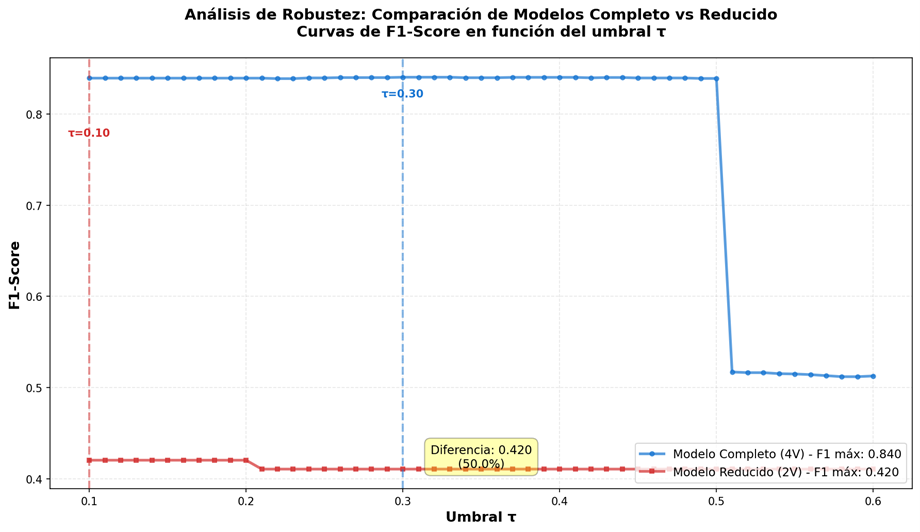
\includegraphics[width=0.9\textwidth]{figuras/analisis_robustez.png}
    \caption{Análisis de robustez: Comparación de rendimiento entre Modelo completo (4 variables) y Modelo reducido (2 variables)}
    \label{fig:analisis_robustez}
\end{figure}

Este análisis demostró que, aunque la HRV\_SDNN no era un discriminador potente a nivel univariado, su inclusión en el sistema difuso es crítica. Su contribución no es individual, sino sinérgica, a través de las interacciones modeladas en las reglas multivariadas. Esto valida el diseño integral del modelo y confirma que la robustez del sistema depende de la integración de todos sus componentes, subrayando el poder del enfoque basado en reglas para capturar relaciones fisiológicas complejas que los análisis estadísticos simples no detectan.

% ============================================================================
\section{Tesis}
\label{sec:tesis}
% ============================================================================

La principal aportación de esta investigación es el desarrollo y la validación de un sistema experto, basado en lógica difusa, capaz de clasificar con alta fiabilidad (F1-Score = 0.840) los patrones de comportamiento sedentario semanal a partir de datos biométricos multivariados, longitudinales y recopilados en condiciones de vida libre. La constatación de la hipótesis de investigación se demuestra al confirmar que el modelo interpretable, fundamentado en reglas de conocimiento clínico, converge significativamente con una clasificación objetiva derivada de un análisis de conglomerados no supervisado. Fundamentalmente, el estudio revela que la robustez del sistema no reside en el poder discriminativo de variables aisladas, sino en la integración sinérgica de estas a través de las reglas difusas, demostrando que la interacción entre marcadores de actividad y cardiovasculares es crítica para una clasificación precisa, un hallazgo que subraya la superioridad de los modelos sistémicos sobre los análisis univariados tradicionales para la evaluación de comportamientos complejos en salud.

\begin{figure}[htbp]
    \centering
    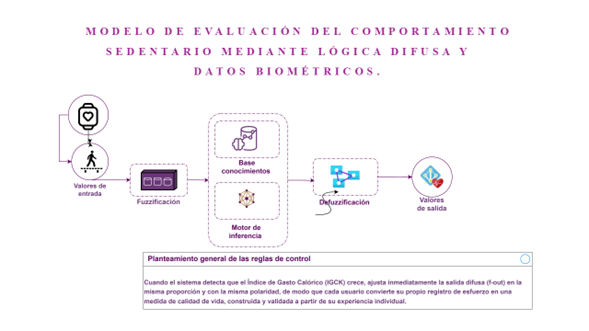
\includegraphics[width=0.95\textwidth]{figuras/diagrama_de_tesis.png}
    \caption{Diagrama conceptual del sistema de evaluación del comportamiento sedentario mediante lógica difusa}
    \label{fig:diagrama_tesis}
\end{figure}
